\begin{frame}{Reward Model (RM)}
  \begin{itemize}
    \item[\textcolor{red}{$\blacktriangleright$}] \textbf{Given:} A prompt $x$ and two responses to it. The annotator marks one as preferred, giving a winner $y_w$ and a loser $y_l$.
    \item[\textcolor{red}{$\blacktriangleright$}] \textbf{Architecture:} Start from the SFT model and replace its next-token output layer with a scalar head, so $r_\phi(x,y)$ returns one score for a prompt-response pair.
    \item[\textcolor{red}{$\blacktriangleright$}] \textbf{Pairwise loss} (the Bradley--Terry preference model):
      \[
      L_{\mathrm{RM}} = -\log \sigma\Big(r_\phi(x, y_w) - r_\phi(x, y_l)\Big)
      \]
      where $\sigma$ is the sigmoid function.
    \item[\textcolor{red}{$\blacktriangleright$}] The loss constrains only the \emph{gap} between the two scores, so the absolute reward scale is arbitrary.
    \item[\textcolor{red}{$\blacktriangleright$}] The RM acts as a proxy for human judgment in downstream RL optimization.
  \end{itemize}
\end{frame}

\begin{frame}{Reward Model Architecture}
  \begin{figure}
    \centering
    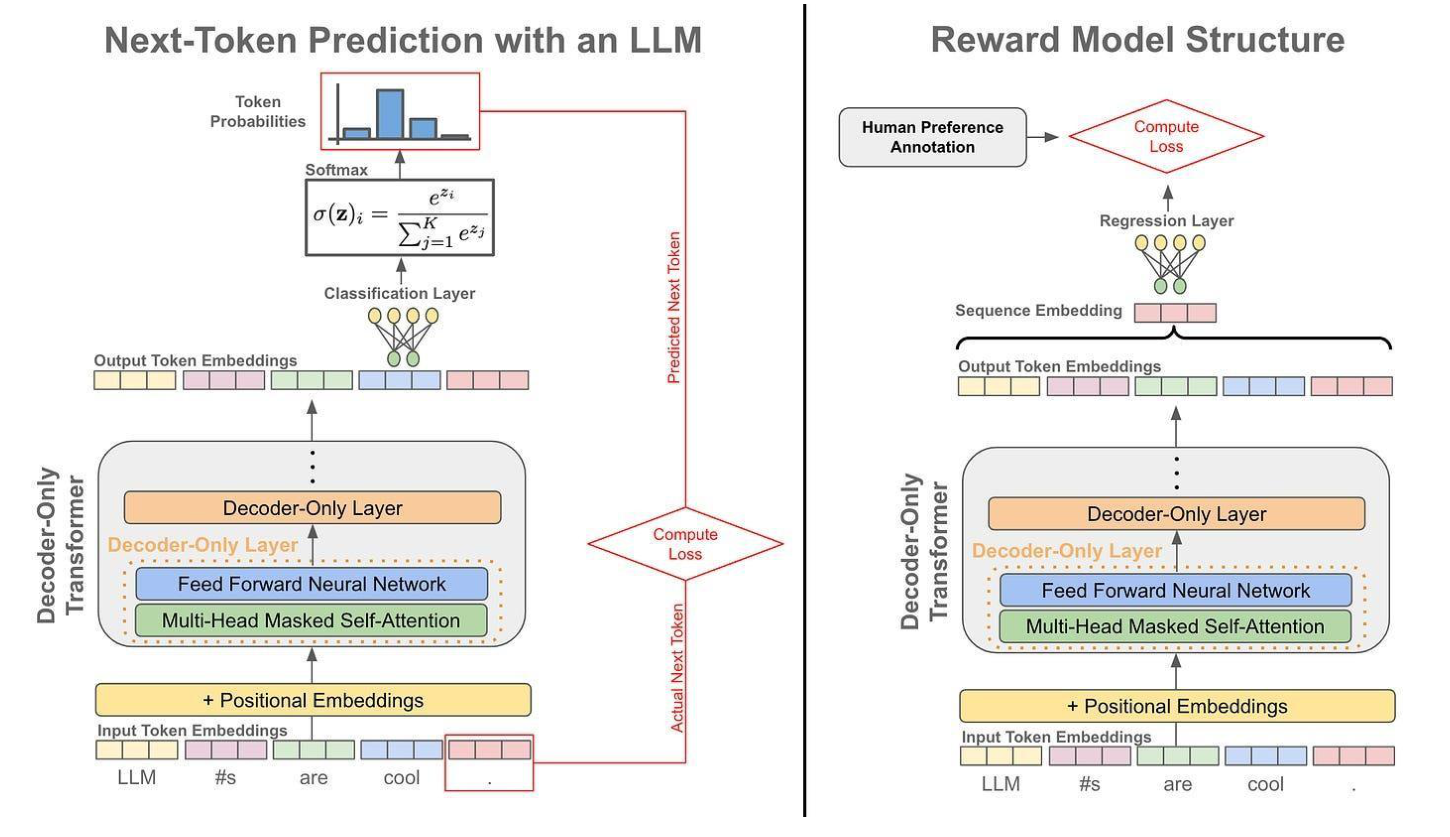
\includegraphics[width=0.74\paperwidth,height=0.60\paperheight,keepaspectratio]{images/llm-rlhf/rlhf_reward_model_structure.png}
    \caption*{\scriptsize Source: Cameron R.~Wolfe, ``The Story of RLHF,'' Deep (Learning) Focus, 2023.}
  \end{figure}
\end{frame}

\begin{frame}{Scoring a Preference Pair}
  \begin{figure}
    \centering
    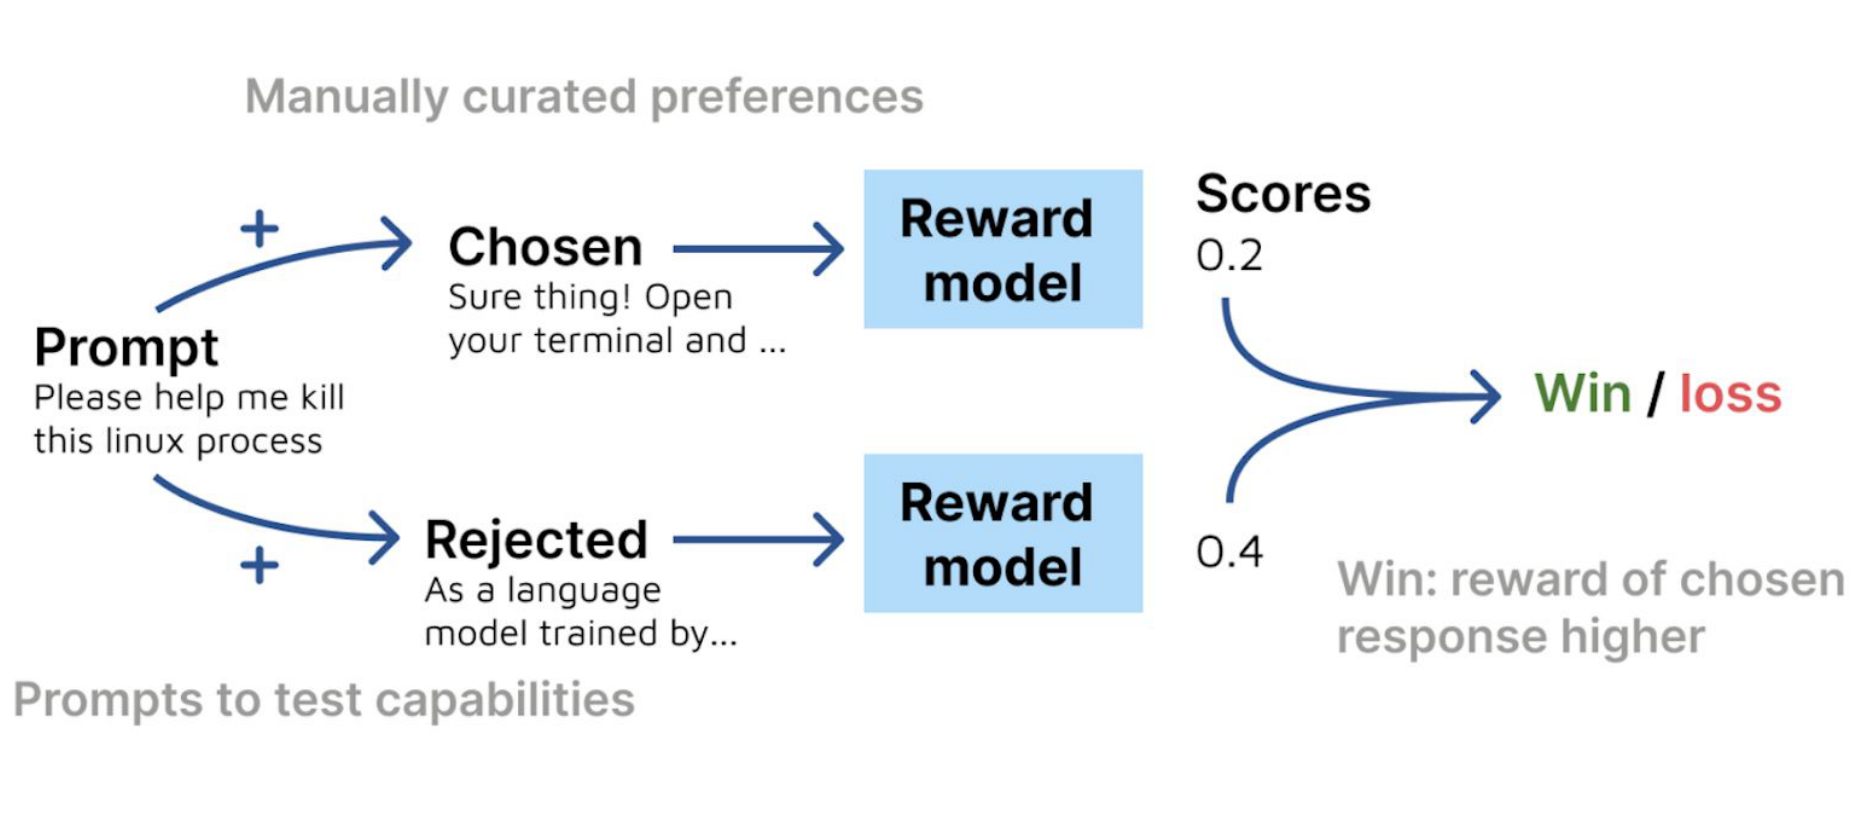
\includegraphics[width=0.74\paperwidth,height=0.60\paperheight,keepaspectratio]{images/llm-rlhf/rlhf_reward_model_preferences.png}
    \caption*{\scriptsize Source: Lambert et al., ``RewardBench: Evaluating Reward Models for Language Modeling,'' 2024, Fig.~1.}
  \end{figure}
\end{frame}
